\documentclass[UTF8]{ctexart}
\usepackage{booktabs}  % professionally typeset tables
\usepackage{amsmath}
\usepackage{setspace}
\usepackage{textcomp}  % better copyright sign, among other things
\usepackage{xcolor}
\usepackage{lipsum}    % filler text
%\usepackage{subfig}
\usepackage{geometry}
\usepackage{float}
\usepackage{hyperref}
\usepackage{graphicx}


%\geometry{left=2.54cm,right=2.54cm,top=2.18cm,bottom=3.18cm}
\date{}
\title{\textbf{通信原理实验}}
\author{无45 \ *** \ **********\\
        无45 \ *** \ **********\\
        无46 \ 黄秀峰 \ 2014011193\\
        无47 \ *** \ **********}


\begin{document}
\maketitle

\section{实验目的}

\section{实验平台}

\section{实验内容}

\subsection{系统功能}

\subsection{系统结构}

\subsubsection{信道编码模块}
卷积码将k个信息比特编码成n个比特,适合以串行形式传。其编码器一般表示为$(n,k,m)$的形式,其中k为每次输入到卷积编码器的比特数,n为每次输入k位比特后输出的编码长度,m为编码存储长度。

本次实验中,我们使用的是$(2,1,3)$卷积编码,每输入一个信息比特,编码产生两位比特的输出,其框图如图.\ref{fig:encoder}所示。

\begin{figure}[htb]
\centering
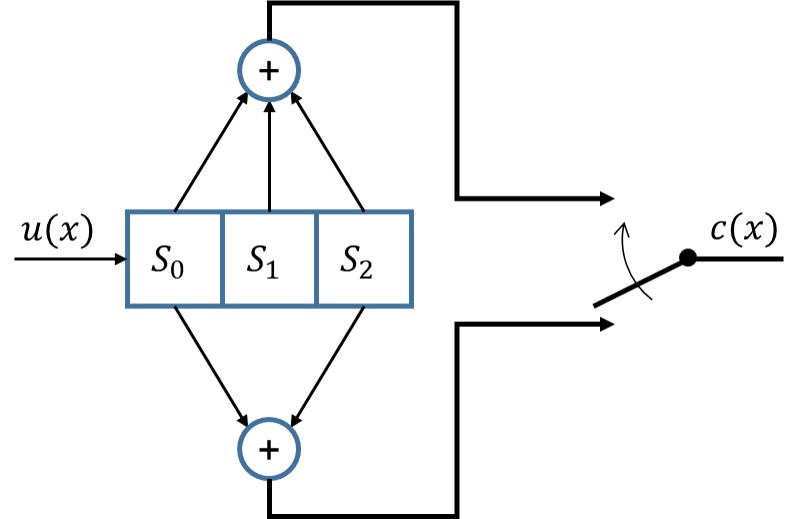
\includegraphics[width=0.4\textwidth]{images//encoder.jpg}
\caption{\label{fig:encoder}(2,1,3)编码器}
\end{figure}

编码器的输入端口信号为:
\begin{itemize}
\item clk\quad        输入控制时钟
\item clk2\quad       输出控制时钟
\item data\_in\quad    编码数据输入
\item reset\quad    重置位
\end{itemize}
其中clk2用于对编码后数据进行控制输出,由于我们采用$(2,1,3)$编码器,故而clk2的频率是clk的两倍。

编码器的输出端口信号为:
\begin{itemize}
\item code\_out\quad        编码数据输出
\item valid\quad       编码有效标志位
\item valid\_wave\quad    编码有效信息流
\end{itemize}
由于我们设计了交织和调制解调模块,需要保证信号同步才能使系统正确工作,所以我们设计了valid以及valid\_wave这两个控制信号来进行各模块间的信号同步。

我们还定义了一个寄存器数组state,用于存储之前时刻的输入。由框图可知,code\_out和state的关系可以表示为:\\
\quad\quad\quad code\_out[0]~=~data\_in + state[0] + state[1]\\
\quad\quad\quad code\_out[1]~=~data\_in + state[1]

每次输入一位比特,编码两位输出,并将valid置为有效。当reset有效时,state清空,并将valid置为无效。

仿真波形如图.\ref{fig:fangzhen}所示。其中data\_send为原始序列,code\_send为编码后序列;二者对应的时钟分别为clk\_div2和clk。从图中可以看出,data\_send每字符占用周期是code\_send两倍。下面用Python检验了一下输出结果,如图
.\ref{fig:PythonSimu},可见我们的编码是正确的。

\begin{figure}[htb]
\centering

\includegraphics[width=0.9\textwidth]{images//encoder_simulation.jpg}
\caption{\label{fig:fangzhen}(2,1,3)编码器仿真波形}
\end{figure}

\begin{figure}[htb]
\centering
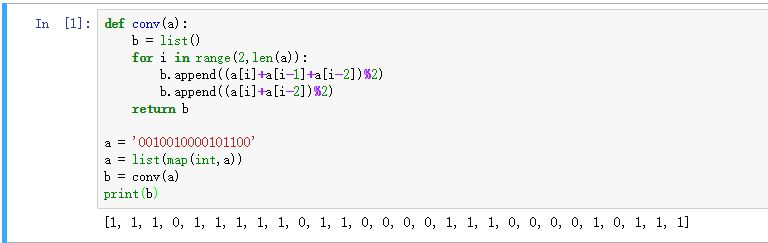
\includegraphics[width=0.8\textwidth]{images//python_simulation.jpg}
\caption{\label{fig:PythonSimu}(2,1,3)编码器输出}
\end{figure}



\subsubsection{交织、解交织模块}

\paragraph{交织器的原理及作用}

在通信中,传输信息比特差错经常是成串发生的。然而,信道编码仅在检测和校正单个差错和不太长的差错串时才有效。为了解决这一问题,希望能找到把一条消息中的相继比特分散开的方法,即一条消息中的相继比特以非相继方式被发送。这样,在传输过程中即使发生了成串差错,恢复成一条相继比特串的消息时,差错也就变成单个(或长度很短),这时再用信道编码纠错功能纠正差错,恢复原消息。简单来说,交织就是将信道传输过程中的连续差错分散化。

\paragraph{交织器的实现}

本实验中采用最常见的交织方法——行列交织。行列交织基本的原理如下图所示:

\begin{figure}[H]
    \centering
    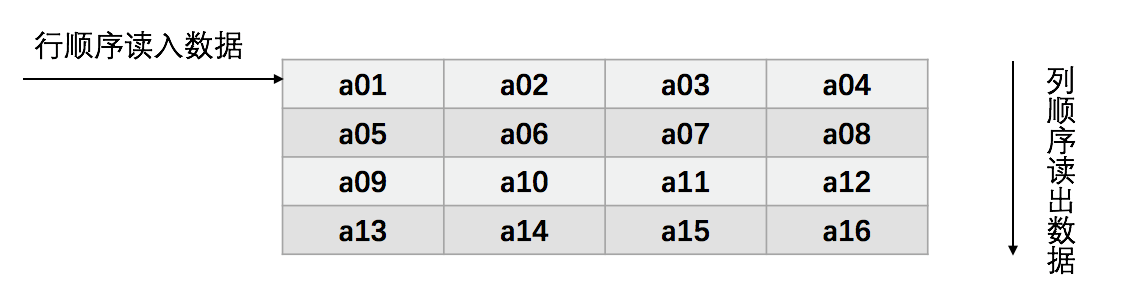
\includegraphics[width=\textwidth]{images//inter_input.png}
\end{figure}

即行顺序写入寄存器,列顺序读出。上图交织结果为a01,a05,a09,a13,a02,a06,a10,a14,a03,a07,a11,a15,a04,a08,a12,a16

解交织时方法和交织相同。

本实验中实现行列交织的具体算法为:

使用两个寄存器数组,一个的作用为行顺序接收当前输入数据并存储时另一个负责按照列顺序输出数组中存储数据。每周期读入一个比特,每16个周期两数组作用互换。

每一周期读入比特的流程图如下:

\begin{figure}[H]
    \centering
    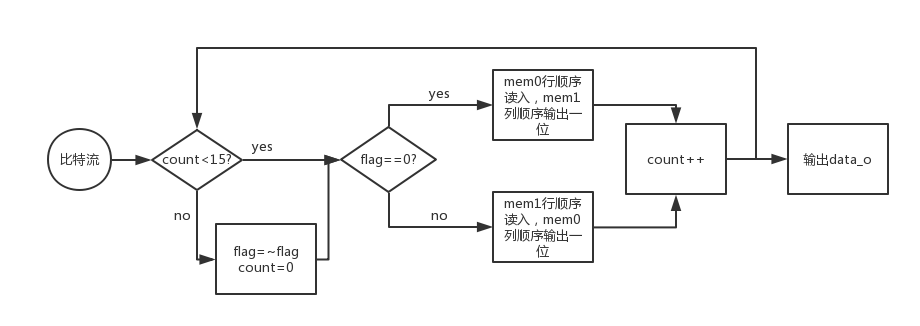
\includegraphics[width=\textwidth]{images//inter_pic.png}
\end{figure}

初始时:count=0;flag=0;mem0[15:0],mem1[15:0]=0;data\_o=0;

\newpage

\subsubsection{调制模块}

\subsubsection{信道模拟模块}

\subsubsection{解调模块}

\subsubsection{信道解码模块}

信道解码使用维特比译码器,判决方式为硬判决。设计思路如下:

\paragraph{变量设计}

\begin{itemize}
\item \textbf{codebuff} : 接收的码流,存于缓冲区中,数量达到一组后送入译码区
\item \textbf{code} : 译码区码流,即当然需要译码的码流
\item \textbf{possible\_codex} : 维特比译码图中,当前阶段第x个状态(共有四个状态)所对应的最优路径
\item \textbf{errorx} : 第x个最优路径(共有4条路径)对应的判决误差
\item \textbf{decodex} : 维特比译码中,当前阶段第x状态的最优路径所对应的输出译码
\item \textbf{decode} : 前一组码流(已译码结束)所对应的输出译码
\end{itemize}

\paragraph{译码流程}

\begin{enumerate}
\item 接收码流至codebuff,当接收完一组后,送入code中等待译码
\item 每一个时钟周期,译码往前推进两位,求出当前状态下的最优路径并计算硬判决误差,并记录四个状态所对应的最优路径
\item 完成一组译码后,将译码结果存入decode,之后每一个时钟周期输出一位译码结果
\end{enumerate}

\subsection{软件仿真}

\section{实验总结}

\end{document}








